\section*{AVL trees%
\TAGS{avl}}

\emph{AVL trees} add an additional invariant in order to ensure the
tree is balanced.  The \emph{height invariant} requires the height of
the left and right subtrees only differ by at most 1. How do we
preserve this invariant? Rotations.

We insert nodes just as we would with a plain BST, but then check to see if
(and where) the height invariant is violated. Say we insert 5 into the
following tree:
\begin{center}
\begin{tabular}{l | r}
  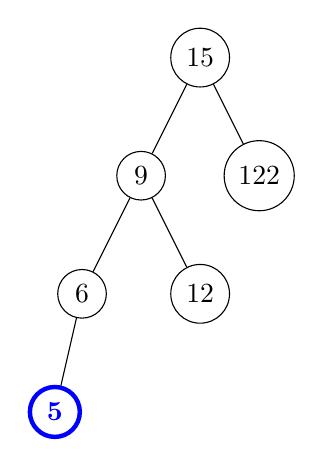
\begin{tikzpicture}
    \tikzstyle{every node}=[circle, draw]
    \node {15} [-]
    child {
      node {9} [-]
      child {
        node {6} [-]
        child[left] {node[blue, ultra thick] {{\bf 5}}}
      }
      child {node {12}}
    }
    child {node {122}};
  \end{tikzpicture}
& 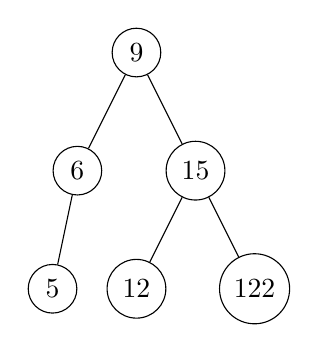
\begin{tikzpicture}
    \tikzstyle{every node}=[circle, draw]
    \node {9} [-]
    child {
      node {6} [-]
      child[left] {node {5}}
    }
    child {
      node {15} [-]
      child {node {12}}
      child {node {122}}
    };
  \end{tikzpicture}
\end{tabular}
\end{center}
Our tree is looking pretty unbalanced. But where is the violation? 6 and 9's
subtrees only differ by 1, but the left subtree of 15 has height 3, while the
right has height 1. To fix this, we rotate {\it right} at 15. Notice that 12
is now the left child of 15, rather than the right child of 9.


Use the visualization at
\url{http://www.cs.usfca.edu/~galles/visualization/AVLtree.html} to insert
$1, 2, 5, 3, 4$ into the tree in the following order, then delete the keys 2
and 4.

\begin{solution}
  \textit{
  Here is a good point to talk about all the rotations. Many people are likely
  confused by double rotations. If you are low on time, it's probably better to
  just skip the checkpoint and explain rotations really well}
\end{solution}


\checkpoint*{\TAGS{avl}}

Now that you've seen rotations, let's write code.

\begin{lstlisting}[name="rotate_right", belowskip=0pt]
tree* rotate_right(tree* T)
//@requires is_tree(T) && T != NULL && T->left !=NULL;
//@ensures is_tree(\result);
{
\end{lstlisting}
\begin{lstlisting}[name="rotate_right", belowskip=0pt, aboveskip=0pt, lineskip=2ex]
  tree* L = [*\answerline{T->left;}*]
  [*\answerline{T->left = L->right;}*]
  [*\answerline{L->right = T;}*]
  [*\answerline{return L;}*]
\end{lstlisting}
\begin{lstlisting}[name="rotate_right", aboveskip=0pt]
}
\end{lstlisting}

The code for \lstinline'rotate_left' is simply the mirror of this function.

\pagebreak

However, sometimes a single rotation is insufficient to rebalance an AVL tree and we need to perform two rotations. Consider inserting 13 into the following tree. Once again our tree is unbalanced at node 15. However, if we rotate right as in the previous example, the tree is still unbalanced!

\begin{center}
\begin{tabular}{l | r}
  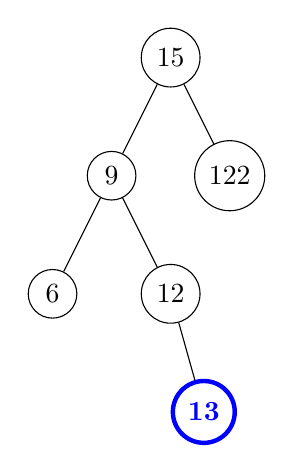
\begin{tikzpicture}
    \tikzstyle{every node}=[circle, draw]
    \node {15} [-]
    child {
      node {9} [-]
      child {
        node {6} [-]
       }
      child {
       node {12} [-]
       child[right] {
         node[blue, ultra thick] {\bf 13}[-]
      }
        }
    }
    child {node {122}};
  \end{tikzpicture}
& 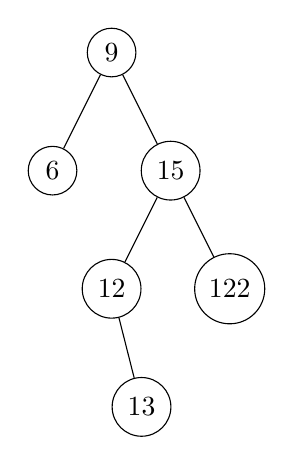
\begin{tikzpicture}
    \tikzstyle{every node}=[circle, draw]
    \node {9} [-]
    child {
      node {6} [-]
    }
    child {
      node {15} [-]
      child {
       node {12} [-]
      child[right] {node{13}}[-]
       }
      child {node {122}}
    };
  \end{tikzpicture}
\end{tabular}
\end{center}


\checkpoint*{\TAGS{avl}}
What two rotations can we perform that will rebalance the above tree? Draw the resulting tree.

\vspace{8cm}

\checkpoint*{\TAGS{avl}}
In general, in what situations is only one rotation necessary? In what situation do we need two rotations?
